% !Mode:: "TeX:UTF-8"
\chapter{帧内无损编码优化算法}
\label{cha:c3}
本章从帧内无损编码的可优化方向的分析开始,引出本研究课题中提出的 3 个优化算法:
1) L 形迭代预测算法 L-IP;
2) L 形分块算法 L-BP;
3) 残差中值边缘检测算法 R-MED。
在具体描述所提出算法之前均先详细地分析了标准规定或 HM 参考软件中的实现方案,以与所提算法形成对比。最后在对各算法性能单独测试的基础上,给出联合算法的性能测试,以证明所提算法的有效性。

\section{帧内无损编码的可优化方向}
当将优化对象聚焦到 H.26X 的帧内无损编码时,编码涉及到的主要模块有:帧内预测模块、熵编码模块以及贯穿编码过程的率-失真优化模块。本课题中提出的 3 个优化算法是在深入分析帧内预测过程及率-失真优化过程后提出的。

对帧内预测模块进行分析。H.26X 的帧内预测是基于块结构进行的,在 H.265 中最小的预测单元大小为 4x4,但针对视频图像中纹理丰富的区域 4x4 大小仍显得有些不足。出于计算复杂度的考虑,H.26X 标准暂时难以跳出块预测的框架,因此寻找更为精准的预测方式是一个可行的优化方向。
块结构的预测准确度仍不够高的原因在于部分被预测点距离参考点的空间距离过大,基于此本课题中提出了 L 形迭代预测算法,在保持整体帧内预测流程仍是块结构的情况下将所有待预测点与参考点的距离缩短到了 1 单位。

对率-失真优化中的 CTU 分割过程进行分析。

对无损模式下帧内预测的残差进行分析。H.26X 中基础的无损编码是通过简单地跳过变换、量化和环路后处理等可能引入数值失真的步骤实现的\upcite{BypassImprovingSCC}。由于缺少了变换这一将数值能量集中的步骤,熵编码面临的压力剧增,既耗时又无法得到理想的编码效率。
但也可以注意到此时待编码数据不再是变换域系数而是预测残差,因此其仍具有空间域的物理意义。
通过进一步分析,发现无损模式下的待编码系数具有不同于自然图像的特殊的空间结构相关性,表现为含有丰富的边缘特征。
基于此本课题中提出了残差中值边缘检测算法 R-MED,对无损模式下的待编码系数进行再处理得到一组能量大幅降低的新待编码系数,以降低熵编码的压力提高整体编码效率。

\section{帧内预测过程分析}
\label{cha:IntraPredDetail}
% 缺失像素的填补方法 参考像素的滤波 模式信息的编码方案 色差通道的异同 不再赘述

\begin{figure}[hbt]
    \centering
    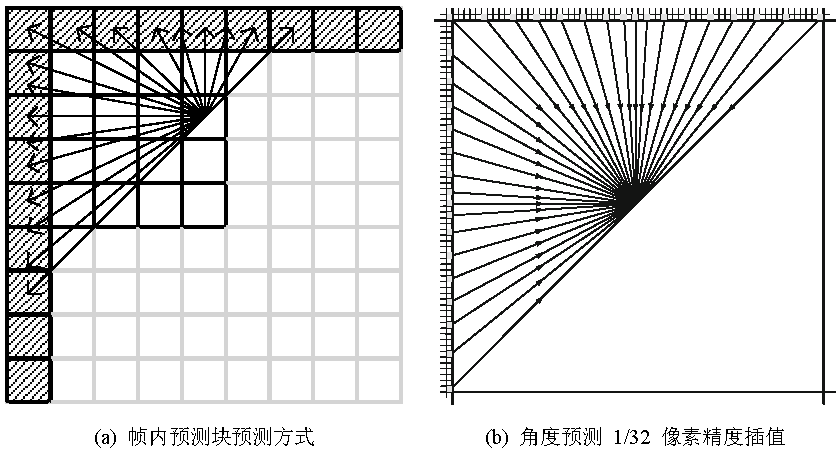
\includegraphics{IntraAngModeOverview.pdf}
    \caption{H.265 帧内预测角度模式}
    \label{fig:IntraAngModeOverview}
\end{figure}

\begin{figure}[hbt]
    \centering
    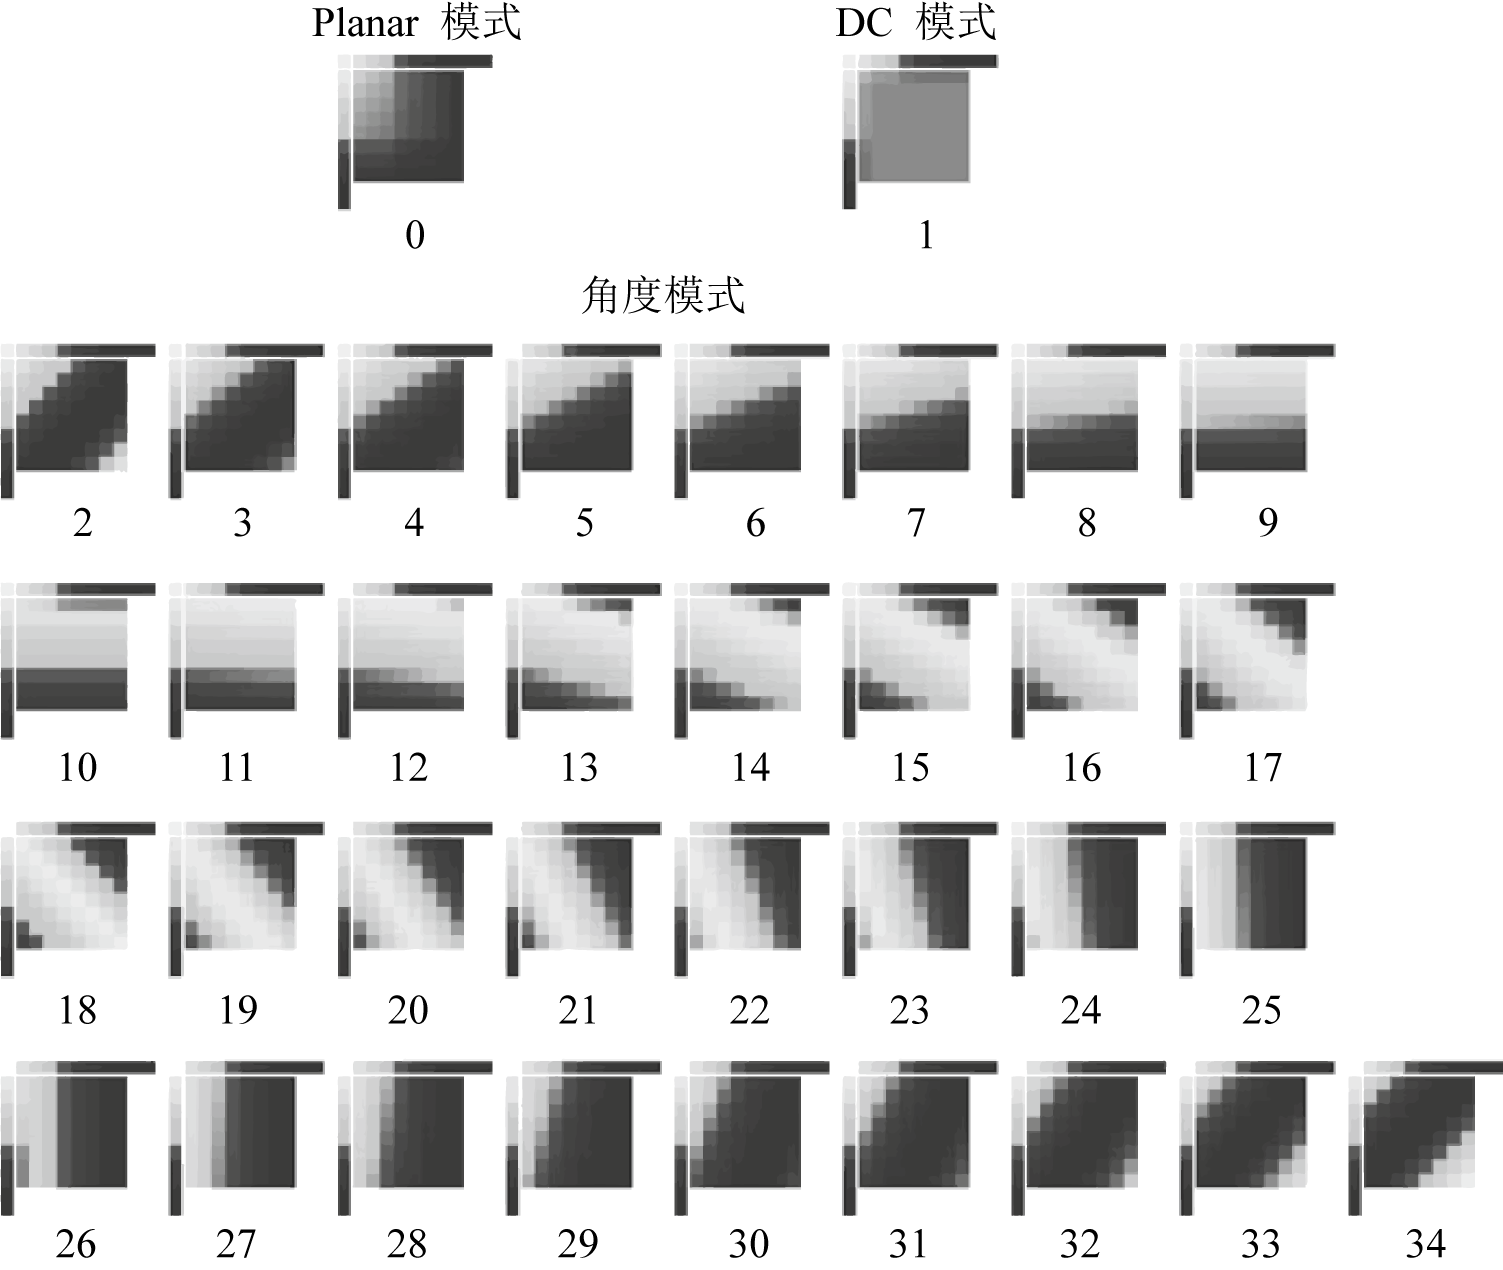
\includegraphics{IntraProjection.png}
    \caption{H.265 帧内预测结果示例}
    \label{fig:IntraProjection}
\end{figure}
% 可能会滤波 所以不是完全投影

\section{帧内无损编码的预测过程优化}

\section{帧内分块决策过程分析}

\section{帧内无损编码的分块过程优化}

\section{系数编码过程分析}

\section{待编码系数的再处理}

\section{联合算法性能测试}